\subsection{Особенности программной реализации генетического алгоритма}
\label{sec:2e}

Генетический алгоритм был реализован в рамках библиотеки PaGMO
(Parallel Global Multiobjective Optimizer) \cite{pagmo}.
Библиотека PaGMO предназначена для решения различных задач оптимизации
и содержит реализации алгоритмов для минимизации одномерных или многомерных,
вещественных или целочисленных целевых функций с линейными или нелинейными
ограничениями. Библиотека написана на языке C++, но также предоставляет
интерфейсы и для языка Python.

Рассматриваемый генетический алгоритм для нахождения равновесной конфигурации
кластера реализован как часть библиотеки PaGMO на языке С++. Все операции с плавающей
запятой выполняются над вещественными числами двойной точности. Программа является
полностью последовательной, то есть не имеет областей кода, выполняющихся параллельно.
Диаграмма классов, которые были задействованы при реализации, изображена на рис. \ref{class_diagram}.
%Использовалась нотация языка UML, представленная в \cite{fowler}

\begin{figure}[ht!]
\centering
  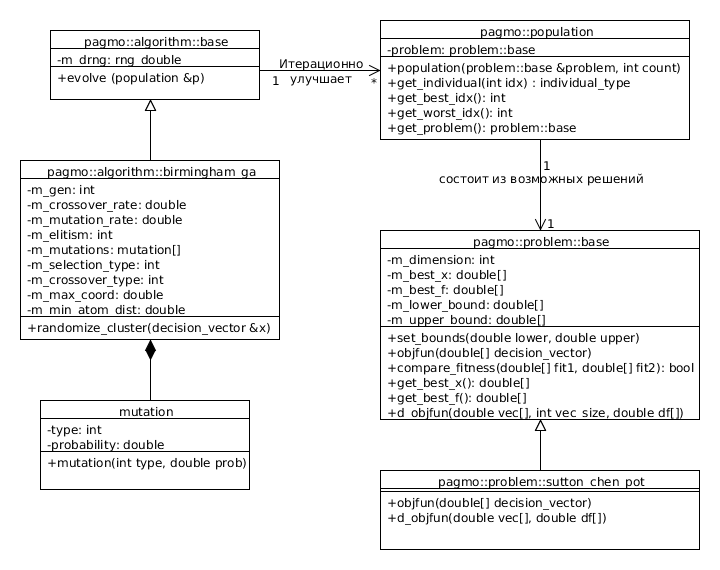
\includegraphics[width=1.0\textwidth]{./FIGs/pagmo_class_hierarchy.png}
  \caption{Диаграмма классов реализации генетического алгоритма}
\label{class_diagram}
\end{figure}

Для сохранения небольших размеров на диаграмме показаны лишь основные поля и методы,
которые были использованы при реализации. Основная логика работы генетического алгоритма
сосредоточена в классе \inlinecode{pagmo::algorithm::birmingham\_ga}. Главным методом
является переопределенный виртуальный метод базового класса \inlinecode{evolve()}.
Он принимает на вход инициализированную некоторым образом популяцию типа \inlinecode{population}.
Класс \inlinecode{population} хранит всю информацию о текущем состоянии популяции:
количество особей, значения хромосом, значения функций приспособленности для каждой из
них, и т.д. Класс \inlinecode{population} также хранит ссылку на оптимизируемую задачу типа
\inlinecode{problem::base}. Этот класс позволяет задать оптимизируемую функцию, а также некоторые её
параметры, в частности верхние и нижние границы значений переменных. Для описания задачи нахождения
равновесной конфигурации металлического нанокластера был создан класс \inlinecode{problem::sutton\_chen\_pot},
являющийся наследником класса \inlinecode{problem::base}. Класс \inlinecode{problem::sutton\_chen\_pot}
переопределяет виртуальные функции \inlinecode{objfun()} и \inlinecode{d\_objfun()}, которые вычисляют
потенциал Саттона-Чена и его градиент для входной конфигурации кластера, соответственно.
Конфигурация кластера представляется одномерным массивом вещественных чисел. Большинству инкапсулированных
членов-переменных класса \inlinecode{algorithm::birmingham\_ga} присваиваются значения во
время конструирования объекта. Эти переменные содержат такие параметры как максимальное количество итераций,
используемые методы скрещивания, селекции и мутации, вероятность мутации и т.д., то есть полностью определяют
поведение генетического алгоритма и во многом дублируют конфигурационные параметры, перечисленные в таблице
\ref{table:iniparams}. Метод \inlinecode{randomize\_cluster()} позволяет сгенерировать новый кластер
со случайными координатами атомов. При этом максимальные координаты атомов в каждом измерении ограничиваются
значением поля \inlinecode{m\_max\_coord}, а минимальное межатомное расстояние задаётся полем
\inlinecode{m\_min\_atom\_dist}.


Параметры для приложения, реализующего генетический алгоритм, задаются в текстовом
инициализационном файле и перечислены в таблице~\ref{table:iniparams}.

%TODO: Make links to chapters with parameters explanation
\begin{table}[H]
\begin{center}
\begin{tabular}{|p{0.25\linewidth}|p{0.75\linewidth}|}
  \hline
  \textbf{Параметр}       &    \textbf{Значение параметра} \\
  \hline
  generations\_number     &    Количество поколений. \\
  \hline
  crossover\_rate         &    Процент особей в новом поколении, произведённых в
                               результате скрещивания. \\
  \hline
  binom\_rate             &    Вероятность обмена отдельных генов в биномиальном методе скрещивания. \\
  \hline
  initial\_rand\_clusters &  Процент кластеров в первом поколении, сгенерированных
                               случайным образом. \\
  \hline
  min\_atom\_dist         &  Минимальное расстояние между атомами в кластере.
                             Используется при генерации кластера со случайными координатами атомов. \\
  \hline
  mut\_move\_rate         &  Вероятность каждого кластера, переходящего в новое поколение, подвергнуться
                             мутации перемещения атомов. \\
  \hline
  mut\_rotate\_rate       &  Вероятность каждого кластера, переходящего в новое поколение, подвергнуться
                             мутации вращения. \\
  \hline
  mut\_replace\_rate      &  Вероятность каждого кластера, переходящего в новое поколение, подвергнуться
                             мутации замены кластера. \\
  \hline
  elitism\_number         &  Если количество прошедших поколений с начала работы алгоритма кратно заданному
                             значению, то кластер с худшим значением функции приспособленности будет заменен
                             на кластер с текущим лучшим значением функции приспособленности среди всех
                             поколений. \\
  \hline
  selection\_type         &  Задает метод, который будет использоваться для выбора родителей для скрещивания. \\
  \hline
  crossover\_type         &  Используемый метод скрещивания: биномиальный или "разрез и склеивание". \\
  \hline
  selection\_type         &  Используемый метод селекции родителей: турнирный или колесо рулетки. \\
  \hline
  bfgs\_step\_size        &  Начальный шаг при поиске вдоль заданного направления в алгоритме BFGS. \\
  \hline
  bfgs\_tol               &  Значение параметра $c_2$ в условиях Вольфе-Пауэлла (\ref{search_constr}) \\
  \hline
\end{tabular}
\caption{Параметры инициализационного файла}
\label{table:iniparams}
\end{center}
\end{table}
